\documentclass{article}

\usepackage{arxiv}

\usepackage[utf8]{inputenc} % allow utf-8 input
\usepackage[T1]{fontenc}    % use 8-bit T1 fonts
\usepackage{hyperref}       % hyperlinks
\usepackage{url}            % simple URL typesetting
\usepackage{booktabs}       % professional-quality tables
\usepackage{amsfonts}       % blackboard math symbols
\usepackage{nicefrac}       % compact symbols for 1/2, etc.
\usepackage{microtype}      % microtypography
\usepackage{lipsum}		% Can be removed after putting your text content
\usepackage{graphicx}
\usepackage{natbib}
\usepackage{doi}
\usepackage{float}
\usepackage{algorithm}
\usepackage{algpseudocode}
% \usepackage{enumitem}
\usepackage[shortlabels]{enumitem}
\usepackage{amsmath,amssymb}
\DeclareMathOperator*{\argmax}{arg\,max}
\DeclareMathOperator{\E}{\mathbb{E}}
\setlist[itemize]{leftmargin=*}



\title{How to not lose your starship: Strategy Optimization for Corellian Spike}

%\date{September 9, 1985}	% Here you can change the date presented in the paper title
%\date{} 					% Or removing it

\author{ Izzie Torres\\
	Department of Aeronautics and Astronautics\\
	Stanford University\\
	\texttt{istorres@stanford.edu} \\
	%% examples of more authors
	\And
	{Maxime Nee} \\
	Department of Aeronautics and Astronautics\\
	Stanford University\\
	\texttt{mdn756@stanford.edu} \\
    %% examples of more authors
 	\And
	{Marta Cortinovis} \\
	Department of Aeronautics and Astronautics\\
	Stanford University\\
	\texttt{martac2@stanford.edu} \\
	%% \AND
	%% Coauthor \\
	%% Affiliation \\
	%% Address \\
	%% \texttt{email} \\
	%% \And
	%% Coauthor \\
	%% Affiliation \\
	%% Address \\
	%% \texttt{email} \\
	%% \And
	%% Coauthor \\
	%% Affiliation \\
	%% Address \\
	%% \texttt{email} \\
}

% Uncomment to remove the date
\date{}

% Uncomment to override  the `A preprint' in the header
\renewcommand{\headeright}{AA 228}
\renewcommand{\undertitle}{Winter 2023 AA 228 Final Project}
% \renewcommand{\shorttitle}{\textit{arXiv} Template}

%%% Add PDF metadata to help others organize their library
%%% Once the PDF is generated, you can check the metadata with
%%% $ pdfinfo template.pdf
\hypersetup{
pdftitle={A template for the arxiv style},
pdfsubject={q-bio.NC, q-bio.QM},
pdfauthor={David S.~Hippocampus, Elias D.~Striatum},
pdfkeywords={First keyword, Second keyword, More},
}

\begin{document}
\maketitle

\begin{abstract}
In this project, we implement a model-free reinforcement learning structure to investigate action optimization for the Star Wars card game, Corellian Spike. The game involves betting credits, buying cards, swapping cards, and rolling dice to become the player with the lowest sum of card values in your hand, winning the credits that have accumulated in the pool. We build a publicly-available Python-based Corellian Spike simulator and model the game as a Markov Decision Process, keeping track of game phase, cards in hand, and credits circulating. We run a batch reinforcement learning algorithm to improve upon an initial policy, implementing an epsilon greedy-inspired exploration method to cover as many reachable common states as possible. Different reward models are tested, and we evaluate the resulting policies against various deterministic ones, as well as how they fare against a human player. Our results show clear improvement in win rate over the random and initial policies. We also evaluate the policies with different amounts of players, showing that a policy trained on a 4-player scenario performs better than the 2-player policy in 8-player games.

\end{abstract}

\section{Introduction} %Izzie
A long time ago in a galaxy far, far away... Lando Calrissian lost the Millenium Falcon to Han Solo in a game of Sabacc. As a used Corellian YT-1300 light freighter, the Millenium Falcon was worth 25,000 credits \cite{starship}.  Years later, Garazeb Orrelios loses an astromech droid (worth around 5000 credits \cite{astromech}) to Calrissian in another game of Sabacc \cite{rebels}. Now, Disney has begun selling Sabacc card decks at Galaxy's Edge so that all fans can have the opportunity to lose equally large amounts of money. Unlike many popular gambling games, Sabacc was popularized fairly recently and has a very niche following. Thus, there are no published optimal strategies and no guidance to potential players. Not only is this a clear gap in public knowledge, but it also leaves players open to losing money when it could have been avoided. The goal of this work is to begin to fill this gap by creating a preliminary optimal policy based on reinforcement learning, which can then be shared with the community at large.

There are many different types of Sabacc to consider. Traditional Sabacc is played with a deck of 76 cards, and has a goal of getting the sum of the cards in your hand as close as possible to 23 \cite{sabacc}. Corellian Spike is a variant of Sabacc which only uses 62 cards and has a goal of getting the sum of cards as close as possible to 0 \cite{spike}. There are four other less common variants, called Jhabacc, Centran Sabacc, Empress Teta preferred style, and Coruscant Shift \cite{sabacc}. The version that is sold at Galaxy's Edge is closest to Corellian Spike, but the rules differ so your hand size can grow from 2 cards to 5 cards, whereas in traditional Corellian Spike you always end the game with 3 cards \cite{spike}. To limit the scope of this project, we will focus on the traditional, canon-accurate Corellian Spike rules, as the Galaxy's Edge version does not explicitly state how betting is handled.

\section{Related Work} %Max
Corellian Spike is a card and dice-based betting game that incorporates elements of other popular games such as blackjack and poker. Though there is no existing literature on optimization strategies for Corellian Spike, numerous studies have been conducted on poker, which has a similar betting mechanic as Corellian Spike. \cite{RW_thesis} applied Q-learning to a simplified variation of poker called UH Leduc poker and showed that the Q-learning trained robot was able to consistently win credits over a large number of hands against both a random agent and a "smart" agent that raised on strong hands, matched on average hands, and folded on weak hands. Blackjack is also similar to Corellian Spike in the way that players are able to gain additional cards that could give them an advantage. \cite{Granville} further validates Q-learning learning by showing that the winnings of a Q-learning trained bot converges to that of the known optimal policy of blackjack.

\section{Problem Statement}
\subsection{Game Mechanics} %Max
To win a hand of Corellian Spike, the player must have the lowest absolute sum of their 3 cards, subject to tiebreaker rules. This non-standard deck consists of 2 zeroes, and 3 of each non-zero number from -10 to 10, inclusive, resulting in 62 cards total. In our project, every player starts a game with 50 credits. A diagram of the game flow is shown in Figure \ref{fig:flowchart}, which further divides the game into 4 distinct rounds, and 3 distinct active decisions. This terminology will be re-introduced in Section 3.2 to define the game model. Each phase of the game is described in more detail below.
\begin{figure}[ht!]
    \centering
    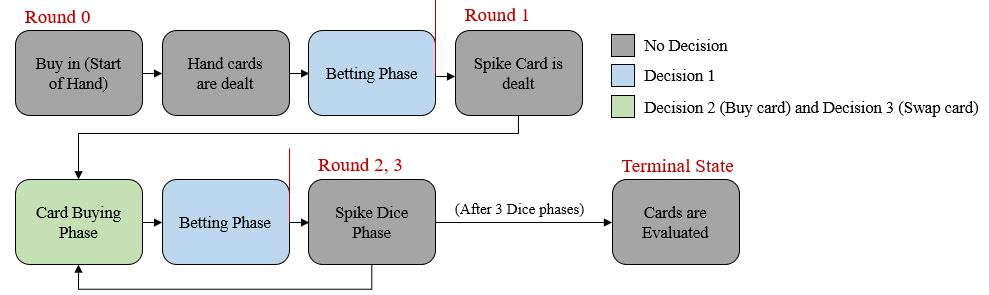
\includegraphics[width=.9\textwidth]{figures/flowchart.jpg}
    \caption{Flowchart of one hand of Corellian Spike}
    \label{fig:flowchart}
\end{figure}
\begin{itemize}
\item \textit{Buy in}$\rightarrow$ players place 2 credits in the pool to buy in and play the next hand. 
\item \textit{Dealing the Hand}$\rightarrow$ after buying in, each player is dealt two cards only for them to see. These cards make up the players' ``hand''.
\item \textit{Betting Phase}$\rightarrow$ the betting phase in Corellian Spike is similar to that of poker where players are not required to make bets until the minimum bet is raised by another player. The minimum bet starts at zero, and can be raised by two credits on a player's turn. The actions available in this phase are match, raise, and fold. When credits are bet, they are added to the pool. If a player folds, they forfeit all the credits they have put into the pool and the game continues without them. They will not be allowed to re-enter the game until the next hand. The betting phase ends after the betting turn returns to the last player who raised. For example, in a three player game, if Player 1 raises, the next two players must either match or fold successively for the betting phase to end. 
\item \textit{Dealing the Spike Card}$\rightarrow$ after the first betting phase, each player who has not folded will be dealt their third card, face up. This card is called the spike card. 
\item \textit{Card Buying Phase}$\rightarrow$ in the card buying phase, each player is given the option to add two credits to the pool to buy a card from the draw pile that they have the option to replace with any of their three cards. The replaced card is moved to the discard pile. A player can also decide to not take the card that they bought and move it to the discard pile instead. A player can also choose not to buy a card.
\item \textit{Spike Dice Rolling Phase}$\rightarrow$ in the spike dice phase, two regular die are rolled. If the dice match, then every player moves both of their hand cards to the discard pile and replaces them with new cards from the draw pile. If the dice are also both ones, the spike card is also replaced.
\item \textit{Evaluating a Winner}$\rightarrow$ if at any point there is only one remaining player who has not folded, that player wins. If the end of the hand is reached without this happening, the player with the lowest absolute sum of their cards wins the hand. If there is a tie, then the cards of the tied players are evaluated subject to these tie-breaker rules, with the lower numbers taking higher priority. 
\begin{enumerate}
    \item The player with the lowest positive sum wins. 
    \item The player with the highest sum of positive cards wins. 
    \item The player with the highest single positive card wins. 
    \item A winner is randomly determined from the tied players.
\end{enumerate}
\end{itemize}

\subsection{Model Definition} %Marta
We modeled a game of Corellian Spike as a Markov Decision Process (MDP). At any point in time, an agent, or player, has full certainty of their cards, credits, and pool, as well as which phase of the game they are in. However, they do not know what opponents have in their hand, nor can they deterministically predict the outcome of spike dice rolls. The most accurate model of this game would include a state space containing every possible combination of rounds, decisions, cards, credits, and pool. This state space is unfathomably large, thus we made simplifications to the model definition to reach a reasonably-sized state space.
\begin{itemize}
    \item \textit{States}$\rightarrow$ we define a state ($s$) based on features available to a player at any point in the game, creating an 8-digit state representation. This representation is shown in Figure \ref{fig:state_digits}.
    \begin{figure}[H]
    \centering
        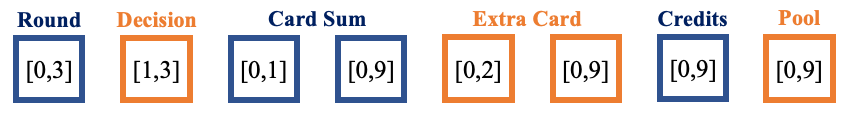
\includegraphics[width=.6\textwidth]{report/figures/state.png}
        \caption{8-digit feature-based state enumeration, with digit ranges}
        \label{fig:state_digits}
    \end{figure}
    As detailed in Section 3.1, there are 4 unique rounds of the game in a single hand, as well as 3 unique decisions. Card sum (two cards in hand plus spike card) is limited to two digits, evaluated by capping the sum to $\pm 9$ and adding 10. The digits of the extra card, or card bought, are found by adding 10 to the value of that card. Finally, both credits and pool are found by dividing the actual values by 10, rounding, and capping the maximum to 9. The actual value of the pool can never exceed the number of all agent credits, reducing the size of the state space. The terminal state, $s=0$, is the state reached at the end of a hand, where the winners are evaluated. This state definition does not include every card in the discard pile, which would have added several orders of magnitude to the size of the state space. Furthermore, bets are limited to 2 credits only. Even then, the size of the state space is 231,041 states for 2 players, and 361,001 for 4.  
    \item \textit{Actions}$\rightarrow$ in total, there are 9 agent actions ($a$), enumerated 0-8 as follows: (0) raise a bet; (1) match a bet; (2) fold; (3) buy an extra card; (4) do not buy an extra card; (5) discard bought card; (6) swap extra card with spike; (7) swap extra card with low value card in hand; (8) swap extra card with high value card in hand.
    \item \textit{Transitions}$\rightarrow$ transitions are modeled exactly following the gameplay detailed in Section 3.1, as given in Figure \ref{fig:flowchart}.
    \begin{enumerate}[a)]
        \item Raising a bet ($a^0$) directly affects an agent's credits and the pool. Depending on rounding artifacts and the order of players, an agent may remain in the same state. Otherwise, an agent could transition to another state with completely different digits, save for the extra card digits. Raising a bet on the last round leads to the terminal state if betting is resolved with a match or fold from the last player. Additionally, the resulting effects of spike dice rolls and the addition of a spike card from round 0 to 1 influence the outcome of raising a bet from one state to the next.
        \item Matching a bet ($a^1$) enables the same transitions as raising a bet. The last player in player order must match or fold to resolve the betting phase.
        \item Folding ($a^2$) enables a deterministic transition to the terminal state.
        \item Buying a card from the draw pile ($a^3$) is the only action that transitions an agent from decision 2 to 3, subtracting credits and adding to the pool accordingly. It also populates the digits reserved for extra card.
        \begin{itemize}
            \item Discarding the card bought ($a^5$) deterministically changes the extra card digits to 0 and shifts decision from 3 to 1.
            \item Swapping with spike card ($a^6$), with low value card ($a^7$), or low value card ($a^8$) updates the sum digits, changes the extra card digits to 0 and shifts decision from 3 to 1.
        \end{itemize}
        \item Not buying a card from the draw pile ($a^4$) shifts decision from 2 to 1, deterministically.
    \end{enumerate}
    \item \textit{Rewards}$\rightarrow$ rewards are driven by credit circulation. Two different reward models were created to assess which one would allow the agent to learn to both win frequently and win a lot of credits. These models are discussed next.
\end{itemize}
We elected to model the game as an MDP rather than a Partially Observable MDP (POMDP) to assess what policy an agent might learn solely based on what they can observe with full certainty. In other words, we were interested in whether an agent could learn to make the most out of their cards without knowledge of what the opponents did or what their hand could be. 
\subsubsection{Reward Model}
Rewards are assigned based on two different models: a credits-only reward model, and a card-sum weighted reward model. The credit-only model assigns rewards only based on the credits spent and gained. Similar to playing against other humans, the credits lost and won drive a player's decision. However, we wanted to further discourage the agent from betting or spending credits if the sum of their cards is high. Therefore, we extended the credit-only model to be weighted with the sum of cards in hand. These models are outlined in Table \ref{tab:rewards}.
\begin{table}[H]
\centering
\caption{Reward Models}
\begin{tabular}{c|c|c}
& \textbf{Credits-only Reward} & \textbf{Weighted Reward}\\ \hline
Raise & -2 & $-2\times (1+|\sum$cards$|)$ \\ \hline
Match& 0 (if no raises), -2 & 0 (if no raises),$-2\times (1+|\sum$cards$|)$ \\ \hline
Buy a card   & -2                       & $-2\times (1+$min(combination of 4 cards)$\times3/4$)\\ \hline
Winning hand & + pool         & +$31\times$pool
\end{tabular}
\label{tab:rewards}
\end{table}
There is no reward associated with losing a hand because the agent has already accumulated negative rewards from betting and buying cards.

\section{Methodology}
For reinforcement learning, agents learn to act in an MDP through experiences in that MDP's simulation environment: by observing state transitions and rewards, an agent learns to choose actions that maximize the total expected reward. The actions ($a$) learned at specific states ($s$) make up a policy, $a = \pi(s)$. To this day, there are no publicly available Corellian Spike simulators. We have created our own Python-based game simulator, which follows the MDP model, complete with state transition data recording. With the data available from the simulator, we apply a model-free, batch reinforcement learning algorithm to explore the state space and let the agent learn to choose favorable actions at various stages of the game. All code used in this report is available in our GitHub repository: \href{https://github.com/martacor2/corellian\_spike}{https://github.com/martacor2/corellian\_spike}.

\subsection{Game Simulator} %Izzie
The simulator was structured as a class called \texttt{CorellianSpike}, with twelve functions for running a hand, playing a series of hands, dealing cards, betting, dealing the spike card, buying a card, rolling the spike dice, evaluating who won, dealing with tiebreakers, getting the state, getting the reward, and recording the data. The cards and credits were tracked using a player dictionary, a deck list, and a pool variable.

The functions for betting and buying a card are most relevant to representing the choices an agent has to make. Betting was modeled as a recursive function. In the first iteration, an agent could choose action 0, 1, or 2. If action 0 (raising) was selected, the function was called again, with arguments changing the minimum bet the next player had to match and which player has the last turn. If actions 1 (matching) or 2 (folding) were selected, the function was called again without these modifications. In the case that the player who chose the action was the last player, the function was not called again, and instead it returned a 2, which indicated to the earlier iterations of the function that betting had ended (for recording purposes).

The buying a card function encompasses two different decisions. First, it checks whether the player wanted to pick action 3 (buy a card) or action 4 (do nothing). Then, if action 3 was selected, it would check if the player wanted to take action 5 (discard), 6 (swap with spike), 7 (swap with low value card in hand) or 8 (swap with high value card in hand).

Recording is handled differently according to different cases. For betting, the action is recorded either when a spike card is dealt or when the spike dice are rolled in order to model the probabilistic state transition that occurs directly after betting. For buying a card and all associated actions, recording is called directly after the action occurred. We tried two different methods of recording wins: one where the last action leads to a terminal state, and another where the last action leads to the first state of the next hand. There was no significant difference in behavior between the two, so we stuck with the former model.

After creating the simulator, we played several games against various policies to check that the game was running the way we expected. We also had the simulator play against itself, then checked the data that was recorded, ensuring the state transitions and rewards were what we expected for each action.

\subsection{Strategy Search} %Marta
We employ Q-learning, which applies incremental estimation of the action value function $Q(s,a)$\cite{228book}. This is a model-free method. Model-based methods require explicit representation of transition and reward models. Since the state space is significantly large, avoiding these explicit representations is highly favorable. $Q(s,a)$ represents the expected return when starting in state $s$, taking action $a$, and then continuing with the greedy policy with respect to $Q$ to the new state $s'$. Mathematically,
\begin{equation}
    Q(s,a) = R(s,a) + \gamma \sum_{s'} T(s' \vert s,a) \max_{a'}Q(s', a')
\end{equation}
where $R$ is the reward model, $\gamma$ is the discount factor, $T$ is the transition model from state $s$ to $s'$ via action $a$, and $a'$ is an available action at state $s'$. The MDP in question is finite horizon, and un-discounted, therefore $\gamma = 1$. This formulation may be written in terms of an expectation over samples of reward $r$ and the next state. By applying the definition of incremental estimation of mean, the $Q$ function is incrementally updated with every new observation as follows:
\begin{equation}
    Q(s,a) \leftarrow Q(s,a) + \alpha \left( r+ \gamma \max_{a'}Q(s',a') - Q(s,a)\right)
\label{eqn:q_update}
\end{equation}
where $\alpha$ is the learning rate. Learning rate influences the rate at which the weights of the older samples decay. For this project, the learning rate has been set to $\alpha = 0.1$. After obtaining $Q(s,a)$, the policy $\pi(s)$ at each state that maximizes the total expected reward is obtained by computing
\begin{equation}
    \pi(s) = \argmax_{a} Q(s,a)
\label{eqn:policy}
\end{equation}
which is also defined as the greedy policy with respect to the value function. By exploring the simulation and gathering a significant amount of data, the Q-learning update will progress the Q-function towards optimum. Exploration was performed via an epsilon greedy-inspired method. 

The learning algorithm for this project functions as follows: we begin with exploration parameter $\epsilon = 0.9$ and decay factor $\alpha_\epsilon = 0.9556$. Then, an initial policy is generated. This is a policy that will always match, always not buy a card, and always discard a bought card at states that allow those actions. This policy was chosen as the initial policy instead of a random policy to avoid a lot of folding at the early stages of learning. With this policy, we let an agent play 2000 games of 10 hands each against other agents running the same policy and record that data. To explore the state space, agents pick with probability $\epsilon$ a completely random allowable action, or pick the action given in the policy for that state with probability $1-\epsilon$. At the end of a set of games, the simulator outputs the transition and reward data, which is passed to a Q-learning function. This function performs the action-value function update from Eq.\ref{eqn:q_update} by looping through the data generated 20 times, ensuring that rewards from higher rounds are propagated back to earlier rounds. A new policy is then generated with Eq.\ref{eqn:policy}, but if a state was not reached in the set of simulations, the previous action to state pair is retained. This process is repeated for a total of 50 iterations, proving the policy outputted from Q-learning as the new simulation policy. The exploration parameter updated with the decay factor ($\epsilon \leftarrow \epsilon\alpha_\epsilon$) to balance exploration with exploitation of good strategies learned as the algorithm progresses. After 50 iterations, $\epsilon = 10.2\%$. At iterations divisible by 5 we output policy text files, as well as the initial policy and the final ``optimal'' policy text files. This algorithm is implemented in Python, and can be found in our \href{https://github.com/martacor2/corellian\_spike}{GitHub repository}.

This algorithm was run for three different cases: 2 players with a credits-only reward model, 2 players with a weighted reward model, and 4 players with a weighted reward model. The performance of these policies generated is analyzed in the following section. It is worth noting that certain parameter choices were made for the sake of runtime. Depending on the computer used to run this iterative algorithm, runtime varied from about 1.5 hours to 10 hours per complete simulation.

\section{Results}
\subsection{Batch Reinforcement Learning Results}
For all three test cases, we generated action distribution plots per saved policy text file. These distributions are evaluated for sets of states divided by round and decision number. These plots are provided in the Appendix section of the report. We noticed that the distribution of actions evidently changes from the initial policy to the one from the fifth learning iteration. However, the distributions settle quite quickly, with little (at most 3\% offset) to no difference in the distributions from one iteration to the next. Given that the state space is significantly big, a large fraction of states that are uncommon are not reached at all, despite the numerous simulations performed with exploration. In that case, the actions of those states remain the same as the ones from the initial policy, skewing the distribution. Furthermore, the simplifications made to reach a reasonably sized state space only keep track of 6 features. Many actual card, credits, and pool combinations are enumerated under the same state, therefore the greedy action learned at that state is derived from a generalized collection of more detailed game features. Finally, exploration diminishes as iterations increase to emphasize exploitation more, which also reduces the number of unique states visited with each iteration.

There are notable observations from the bar graphs in the Appendix. As iterations progress, the policy learned increasingly favors raising in round 0 of the game for all test cases (Figures \ref{fig:dec1_distribution}, \ref{fig:weight_dec1_distribution}, and \ref{fig:4p_dec1_distribution}). This increase is more evident in the four player test case, where the raising distribution settles around 48\% for all round 0 betting states. Raising is generally more common in a two player setting with a card sum weighted reward model than a credit-only model. For other betting rounds, the policies appear to heavily favor matching for all test cases. For example, raising occurs for about 2\% on average for all rounds of betting related states in a two player setting, which corresponds to about 500 unique states. Furthermore, the policy of all test cases include folding for less than 1\% of the betting-specific state space.

Although quite small, the ``buy card'' action distribution for decision 2 across all cases (Figures \ref{fig:dec2_distribution}, \ref{fig:weight_dec2_distribution}, and \ref{fig:4p_dec2_distribution}) increases with iterations. The agent appears to have learned that spending credits to buy an extra card can lead to winning a favorable sum of credits at the end. Finally, the policies related to decision 3 (Figures \ref{fig:dec3_distribution}, \ref{fig:weight_dec3_distribution}, and \ref{fig:4p_dec3_distribution}) never elect to swap the extra card bought with the high value hand card. This is true for all test cases. Again, this is likely an artifact of the simplified state model, which does not actually capture individual card values.

Action distributions offer insight into what an agent learned to do throughout the iterative algorithm. However, we cannot know if the agent learned to win games and credits from distributions alone. Policy evaluation with various success metrics for the different test cases is discussed next.

\subsection{Policy Evaluation} %Izzie
After obtaining a final ``optimal'' policy from Q-learning, we ran 2000 simulated games of 10 hands against a random policy, the initial policy we started Q-learning with, and an intermediate policy from just 25 iterations. We also tested one game of 10 hands against a human player (the recorded bust occurred in the last hand). The results the 2-player credits-only reward model test case are summarized in Table \ref{tab:results1}.
\begin{table}[H]
\centering
\caption{Performance of Policy with Credits-only Reward Model}
\begin{tabular}{ c | c | c | c | c | c | c }
 \textbf{Metric} & \multicolumn{2}{|c|}{\textbf{Average Credits Won}} & \multicolumn{2}{|c|}{\textbf{Win Rate}} & \multicolumn{2}{|c}{\textbf{Bust Count}} \\ \hline 
 \textbf{Opponent}  & \textit{Opponent} & \textit{Optimal} & \textit{Opponent} & \textit{Optimal} & \textit{Opponent} & \textit{Optimal} \\ \hline
 %Random Policy & -34.7 & 34.7 & 8\% & 92\% & 341 & 1 \\  
 Random Policy & -35.6 & 35.6 & 10\% & 90\% & 499 & 0\\
 %Initial Policy & 3.4 & -3.4 & 37\% & 63\% & 0 & 22 \\
 Initial Policy & 2.4 & -2.4 & 36\% & 64\% & 0 & 17 \\
 %Intermediate Policy & -1.4 & 1.4 & 55\% & 45\% & 180 & 125 \\
 Intermediate Policy & -1.0 & 1.0 & 51\% & 49\% & 180 & 151 \\
 %Win Games Policy & 1.1 & -1.1 & 55\% & 45\% & 565 & 573\\
 Human  & 50 & -50 & 80\% & 20\% & 0 & 1 \\
\end{tabular}
\label{tab:results1}
\end{table}
A few things are notable about this data. First, the optimal policy far outperforms the random policy. It also wins more than the initial policy, but slightly loses in credits. With the intermediate policy, both metrics are near equal. This is to be expected, given the distributions of actions discussed in the previous section. The human also far outperforms the simulator, but the human has some natural advantages as well. For example, the human can see what the other player's spike card is, but we do not include the other player's spike card in our state representation. That choice was made due to the size of our state space, but it also limits the agent's ability to beat a human. Similarly, the state space representation only includes the sum of all the cards, not what the individual cards are. A human can use the knowledge of what their individual cards are to reason about if they are likely to get a card with a lower or higher value in the buying phase. They can also use that knowledge in deciding how to swap an extra card with the cards in their hand. However, the current state space model impedes access to all this information. Finally, a human can also remember what cards have already been drawn, allowing them to reason about what cards are likely to appear. In fact, the simulator displays information about every round, so the human does not have to rely on their own memory. The agent, however, does not take into account the previous cards that have been seen in the state representation. With all of these human advantages, it is somewhat impressive that we can beat the human 20\% of the time through Q-learning.

We also performed this analysis in a 2-player setting for the weighted reward model. These results are summarized in Table \ref{tab:results2}. Note that in this table, the human played four games with a maximum of 10 hands, but the high frequency of busts meant that only 11 hands total were played.

\begin{table}[H]
\centering
\caption{Performance of Policy with Weighted Reward Model}
\begin{tabular}{ c | c | c | c | c | c | c }
 \textbf{Metric} & \multicolumn{2}{|c|}{\textbf{Average Credits Won}} & \multicolumn{2}{|c|}{\textbf{Win Rate}} & \multicolumn{2}{|c}{\textbf{Bust Count}} \\ \hline 
 \textbf{Opponent}  & \textit{Opponent} & \textit{Optimal} & \textit{Opponent} & \textit{Optimal} & \textit{Opponent} & \textit{Optimal} \\ \hline
 Random Policy & -38.4 & 38.4 & 5\% & 95\% & 624 & 1 \\
 Initial Policy & 0.1 & -0.1 & 37\% & 63\% & 157 & 208 \\
 Intermediate Policy & 0.8 & -0.8 & 51\% & 49\% & 891 & 906 \\
 Human & 25 & -25 & 73\% & 27\% & 1 & 3 \\ 
 % 2 hands -50, lost twice, busted once
 % 3 hands +50, won twice, other person busted
 % 4 hands +50, won four times, other person busted
 % 2 hands +50, won twice, other person busted
Credits-only Policy & -0.6 & 0.6 & 46\% & 54\% & 555 & 569 \\
\end{tabular}
\label{tab:results2}
\end{table}

The results are fairly similar to the policy formed by the other reward model. Thus, we conclude that by using the reward function solely based on credits bet and won, we save some lines of code and conceptual complexity for a very slight impact on learning capabilities.

\subsection{Policy Evaluation with more than 2 players}
Next, we compared a policy generated for a 4-player scenario to the 2-player policy obtained with a weighted reward model. As the number of players in a game increases, the total amount of money and the number of potential winners increases, which we expect to impact the optimal strategy. The results are summarized in Table \ref{tab:resultsMulti}.
\begin{table}[H]
\centering
\caption{Multi-Player Performance in Various Scenarios}
\begin{tabular}{ c | c | c | c | c | c | c }
\textbf{ Metric} & \multicolumn{2}{|c|}{\textbf{Average Credits Won}} & \multicolumn{2}{|c|}{\textbf{Win Rate}} & \multicolumn{2}{|c}{\textbf{Bust Count}}\\ \hline
 \textbf{Number of Players} & \textit{2-player} & \textit{4-player} & \textit{2-player} & \textit{4-player }& \textit{2-player} & \textit{4-player} \\ \hline
 2 & 18.3 & -18.3 & 64\% & 36\% & 329 & 1044 \\  
 4 & 1.7 & -1.6 & 27\% & 26\% & 575 & 619 \\
 8 & -1.2 & 1.0 & 12\% & 14\% & 0 & 0 \\
\end{tabular}
\label{tab:resultsMulti}
\end{table}
As expected, the policy trained for a 2-player setting outperforms the 4-player policy in a 2-player setting. Unexpectedly, however, it also matches the 4-player policy for performance in a 4-player setting, despite not being trained for that setting and having been trained on fewer lines of data overall (as a result of 4-player simulations generating more lines for the same number of simulations). However, the 4-player policy does start to outperform the 2-player policy in an 8-player setting. We believe this is because the previously mentioned differences in game dynamics due to an increase in players are exaggerated in the 8-player setting. While the differences might have been too slight to afford the 4-player an advantage in a 4-player setting, the 4-player policy better extrapolates to the 8-player setting that neither policy was trained on.
%number of players is the setting, not the policy
%\subsection{Learning by running one hand and change the reward function so that you don't lose your starship}
%adding negative reward (-50 doubles their potential maximum losses)
\section{Conclusion}
In this project we modeled Corellian Spike as an MDP and applied Q-learning to find the optimal policy to win as frequently as possible and as much money as possible. Due to the size of the state space, we chose to learn with a model-free method to avoid explicit representations of our transition and reward models. For this reason, we found Q-learning to be a good fit for our project. 
We found that our optimal policy, which was generated after 50 iterations of Q-learning, far outperformed a random policy, winning an average of 35.6 credits over 10 hands and over 90\% of the time. However, we saw that our intermediate policy, generated after 25 iterations, performed equally well as our optimal policy. Our optimal policy loses consistently to a human player, though the human player has the advantage of being able to observe more states, as well as the actions of their opponent.

Future avenues of improvement to this work include modeling the game as a Partially Observable MDP (POMDP), establishing a belief over the opponent's hand based on observations of their spike card and the cards they discard. Reworking the state space to give full knowledge of the values each of the 3 cards instead of a combined sum could also lead to a better swapping policy, though the state space would grow considerably. A possible solution to this would be to remove the credit aspect of the game and focus on finding the optimal strategy for obtaining the best hand. We could also implement more rules, such as special hands that trump regular hands, or analyze the effect of cheating (addition of a secret fourth card that a player can swap before evaluating cards) on win rate.
\section*{Acknowledgements}
We would like to thank Dr. Kochenderfer and the teaching staff for their continued support throughout the quarter.
\section*{Contributions of Team Members}
\begin{table}[H]
    \begin{center}
    \caption{Contributions Table}
    \begin{tabular}{ p{1in} | p{5in} } 
        \textbf{Group Member} & \textbf{Contribution to Project} \\  \hline
        Izzie Torres (4 credits) & Wrote run\_hand, play\_sabacc, bet, get\_state, get\_reward, and record functions for simulator; adapted simulator to play against a human; adapted simulator to play with different policies for each player; wrote code to generate a random policy; ran learning algorithm for 4-players and an alternative method for recording data; ran simulations for policy evaluation; authored sections 1, 4.1, 5.2, and 5.3; co-authored abstract\\ \hline
        Maxime Nee (3 credits)& Wrote spike\_dice, buy\_card for simulator; ran q-learning for credits-only policy; gathered human vs credits-only reward policy data; authored sections 2, 3.1, 6\\ \hline
        Marta Cortinovis (3 credits) & Wrote tie\_breaker, evaluate\_hands and deal\_card for simulator; wrote batch reinforcement learning algorithm  code as described in the report; ran learning algorithm for 2-players  with weighted reward model; authored sections 3.2, 3.2.1, 4.2, 5.1; co-authored abstract\\
    \end{tabular}
    \end{center}
\end{table}

% \section*{Contributions of Team Members}
% \begin{table}[H]
%     \begin{center}
%     % \caption{Contributions Table}
%     \begin{tabular}{ | p{2in} | p{4in}| } 
%         \hline
%         \textbf{Group Member} & \textbf{Contribution to Project} \\  \hline
%         Mira Partha & Performed literature survey on data-driven detection strategies; collaborated on developing parsing routines for TEXBAT; developed and analyzed support vector machine detection; authored sections 2, 5.2, 6.2; co-authored sections 1, 3, 7\\ \hline
%         Marta Cortinovis & Performed literature survey on theory-driven detection strategies; collaborated on developing parsing routines; developed and analyzed received power monitoring detection; authored sections 5.1, 4, 6.1; co-authored sections 1, 3, 7\\ \hline
%     \end{tabular}
%     \end{center}
% \end{table}
\section*{Appendix}
\subsubsection*{Policy Distribution Plots Credits-only Reward Model and Two Players}
    \begin{figure}[H]
    \centering
        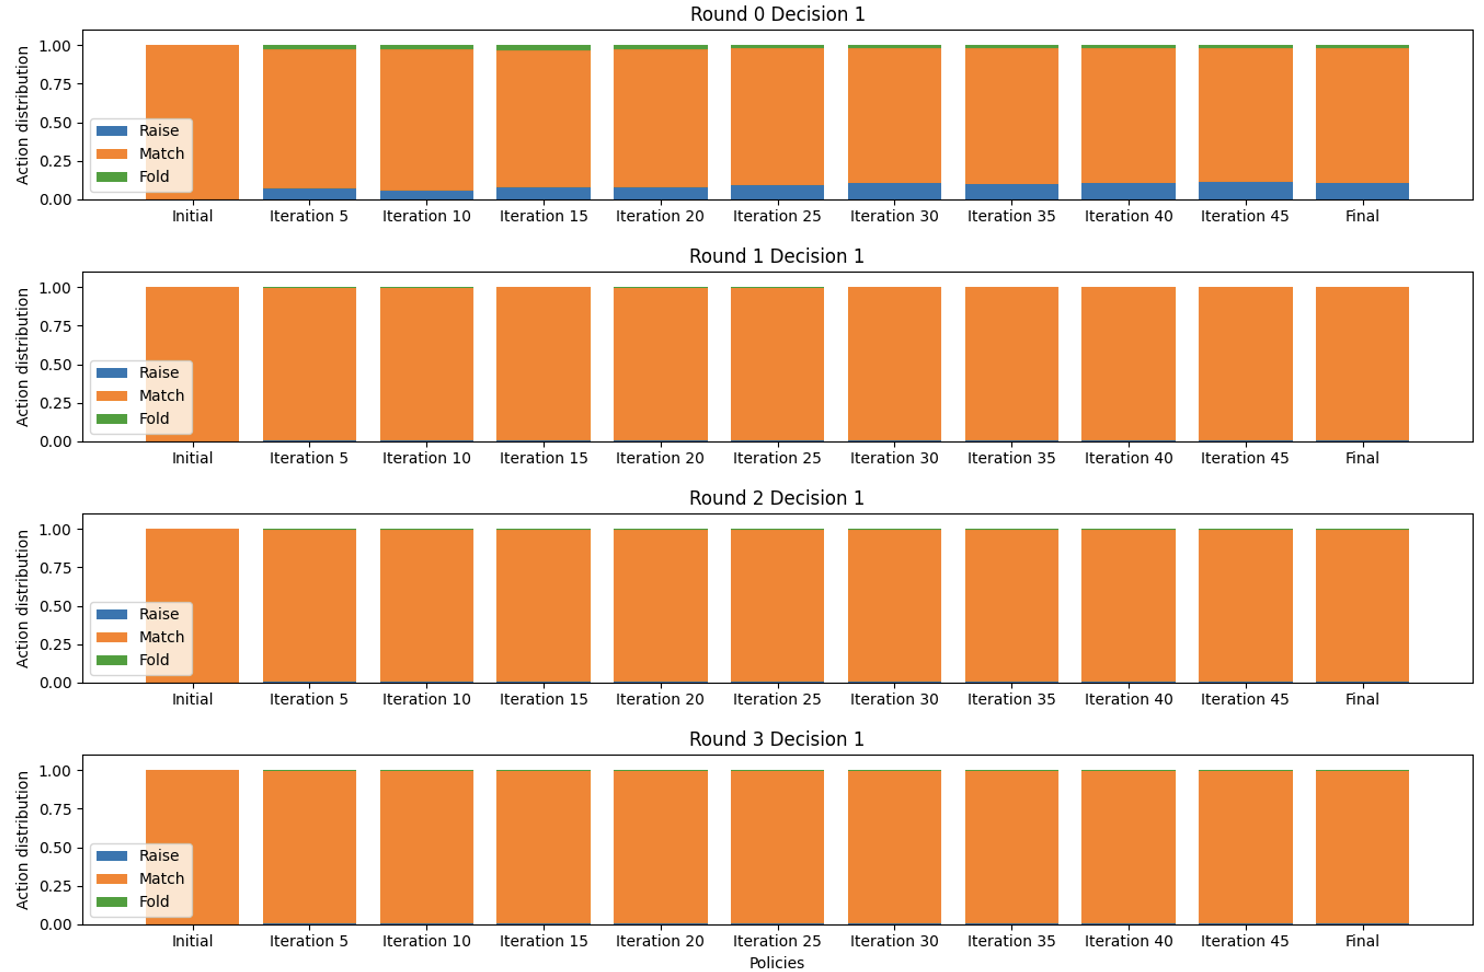
\includegraphics[width=\textwidth]{report/figures/r_d1.png}
        \caption{Action distribution for different policy iterations at Decision 1 with Credits-only Reward Model and 2 players}
        \label{fig:dec1_distribution}
    \end{figure}
    
    \begin{figure}[H]
    \centering
        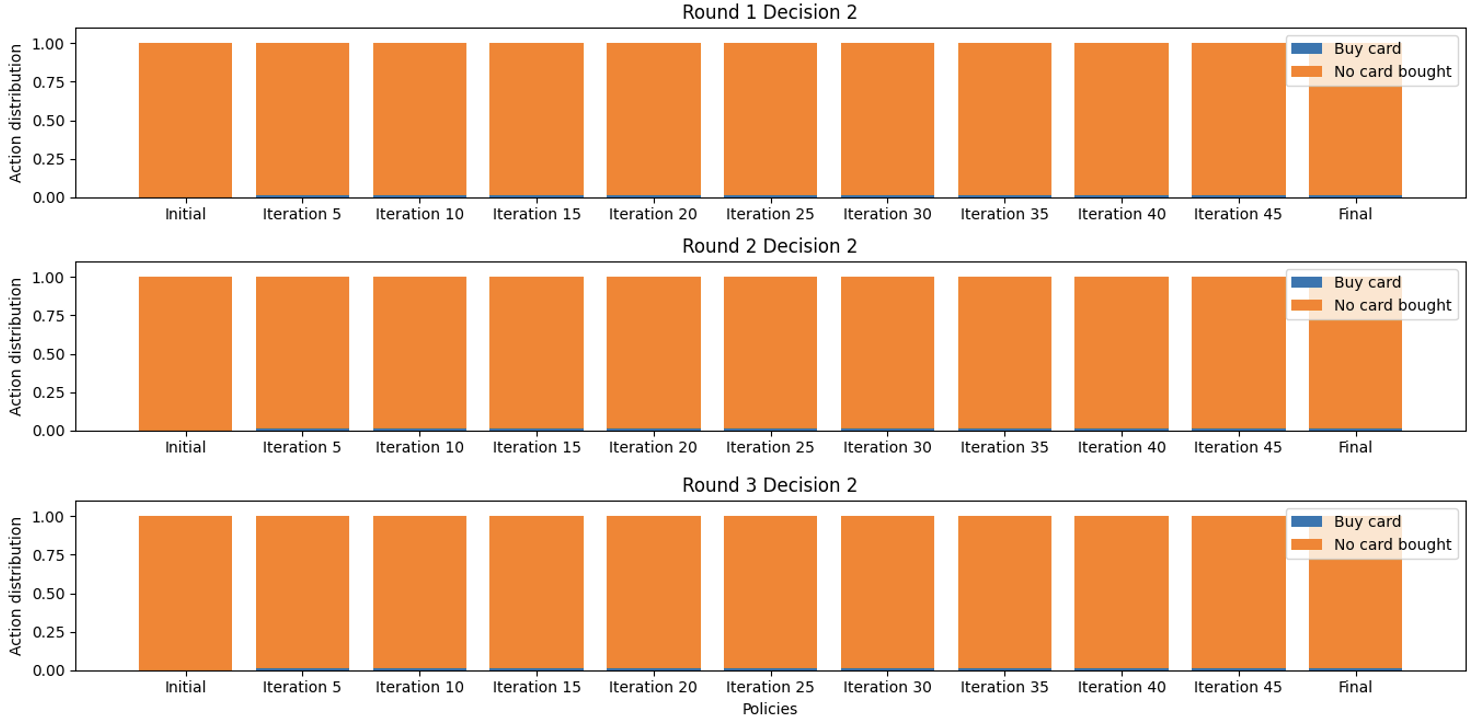
\includegraphics[width=\textwidth]{report/figures/r_d2.png}
        \caption{Action distribution for different policy iterations at Decision 2 with Credits-only Reward Model and 2 players}
        \label{fig:dec2_distribution}
    \end{figure}
    
    \begin{figure}[H]
    \centering
        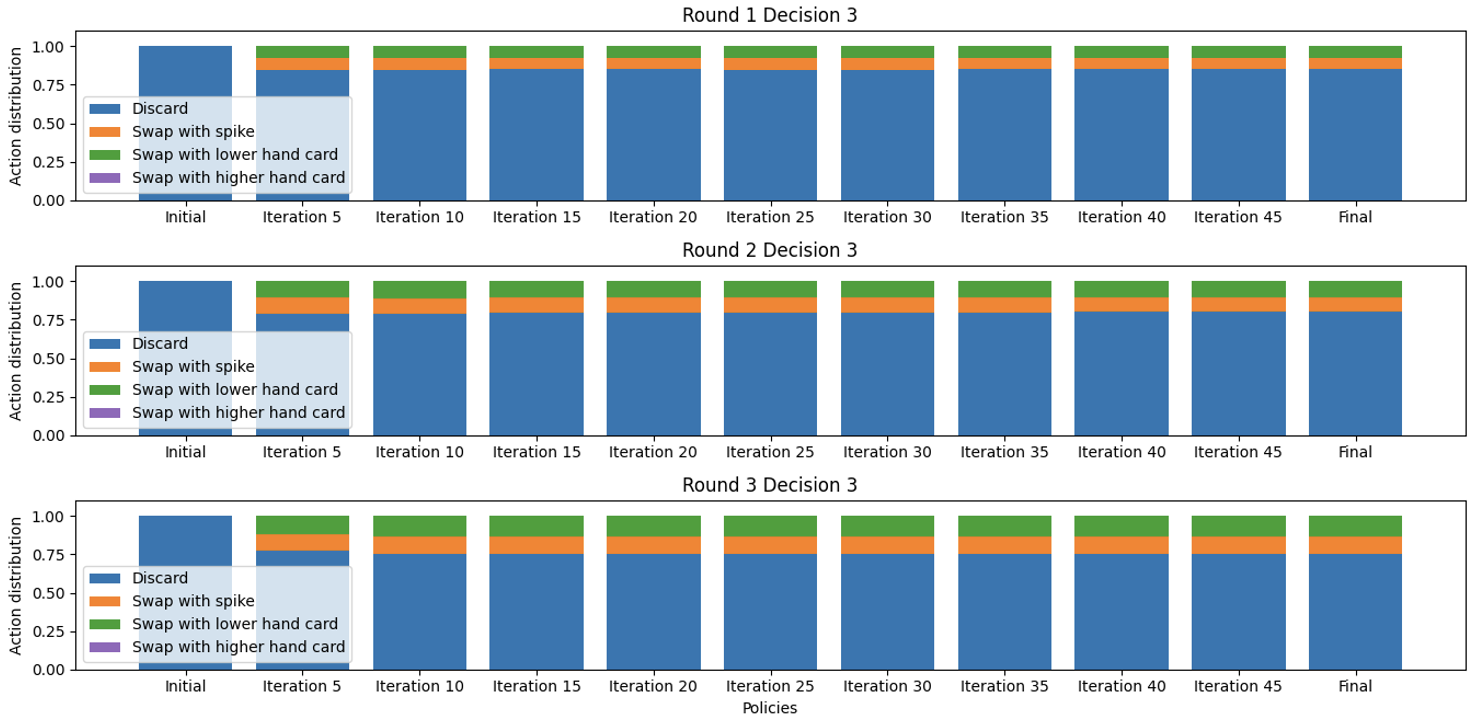
\includegraphics[width=\textwidth]{report/figures/r_d3.png}
        \caption{Action distribution for different policy iterations at Decision 3 with Credits-only Reward Model and 2 players}
        \label{fig:dec3_distribution}
    \end{figure}

\subsubsection*{Policy Distribution Plots Weighted Reward Model and Two Players}
    \begin{figure}[H]
    \centering
        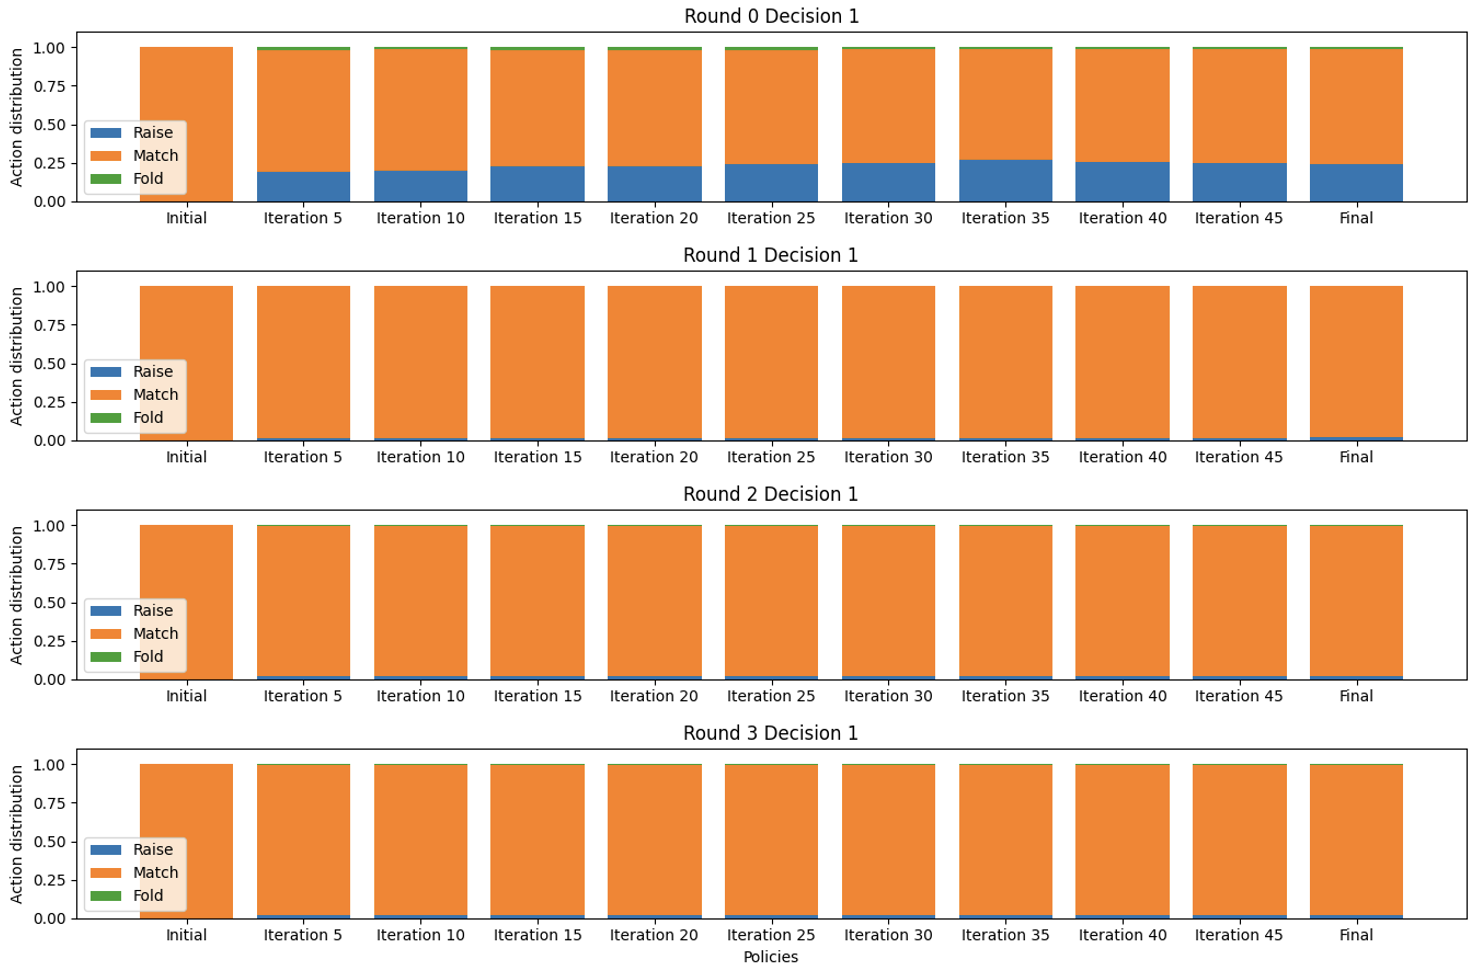
\includegraphics[width=\textwidth]{report/figures/weighted_r_d1.png}
        \caption{Action distribution for different policy iterations at Decision 1 with Weighted Reward Model and 2 players}
        \label{fig:weight_dec1_distribution}
    \end{figure}
    
    \begin{figure}[H]
    \centering
        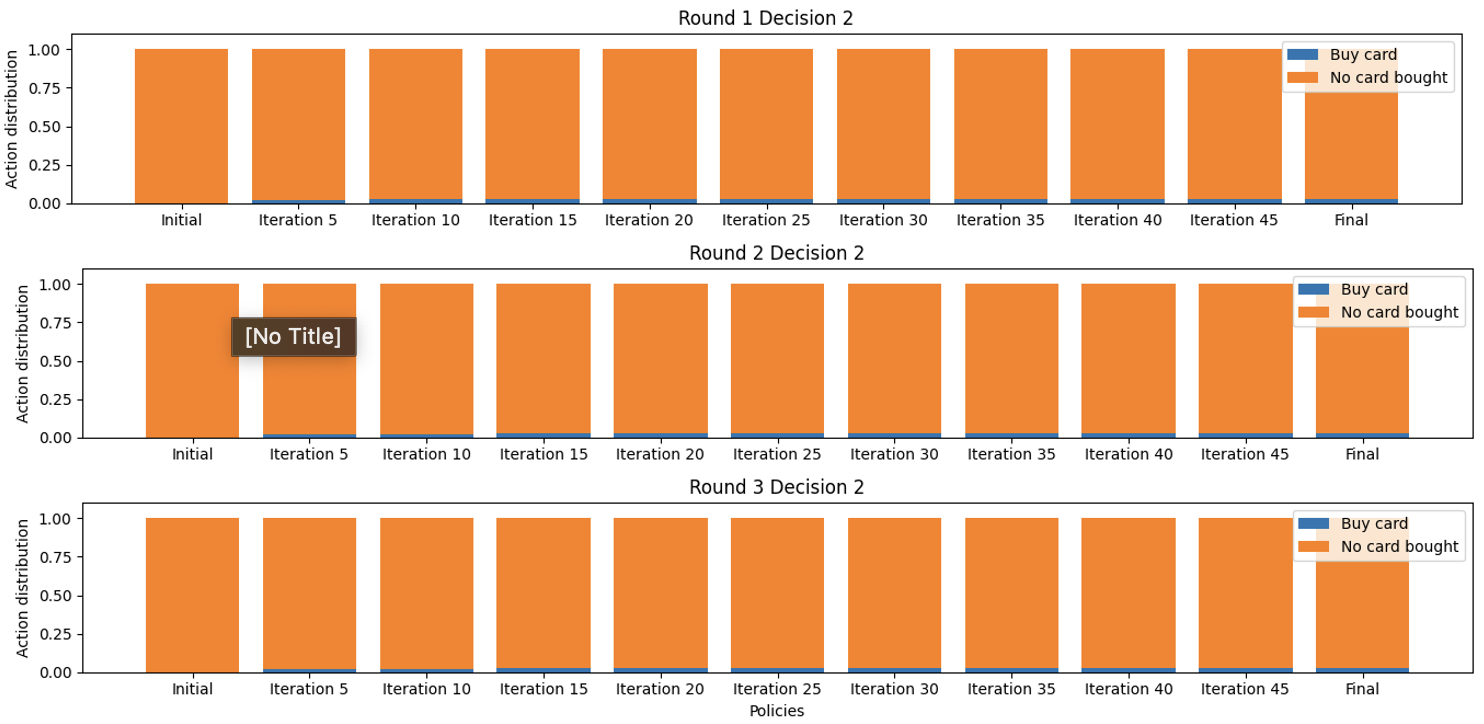
\includegraphics[width=\textwidth]{report/figures/weighted_r_d2.png}
        \caption{Action distribution for different policy iterations at Decision 2 with Weighted Reward Model and 2 players}
        \label{fig:weight_dec2_distribution}
    \end{figure}
    
    \begin{figure}[H]
    \centering
        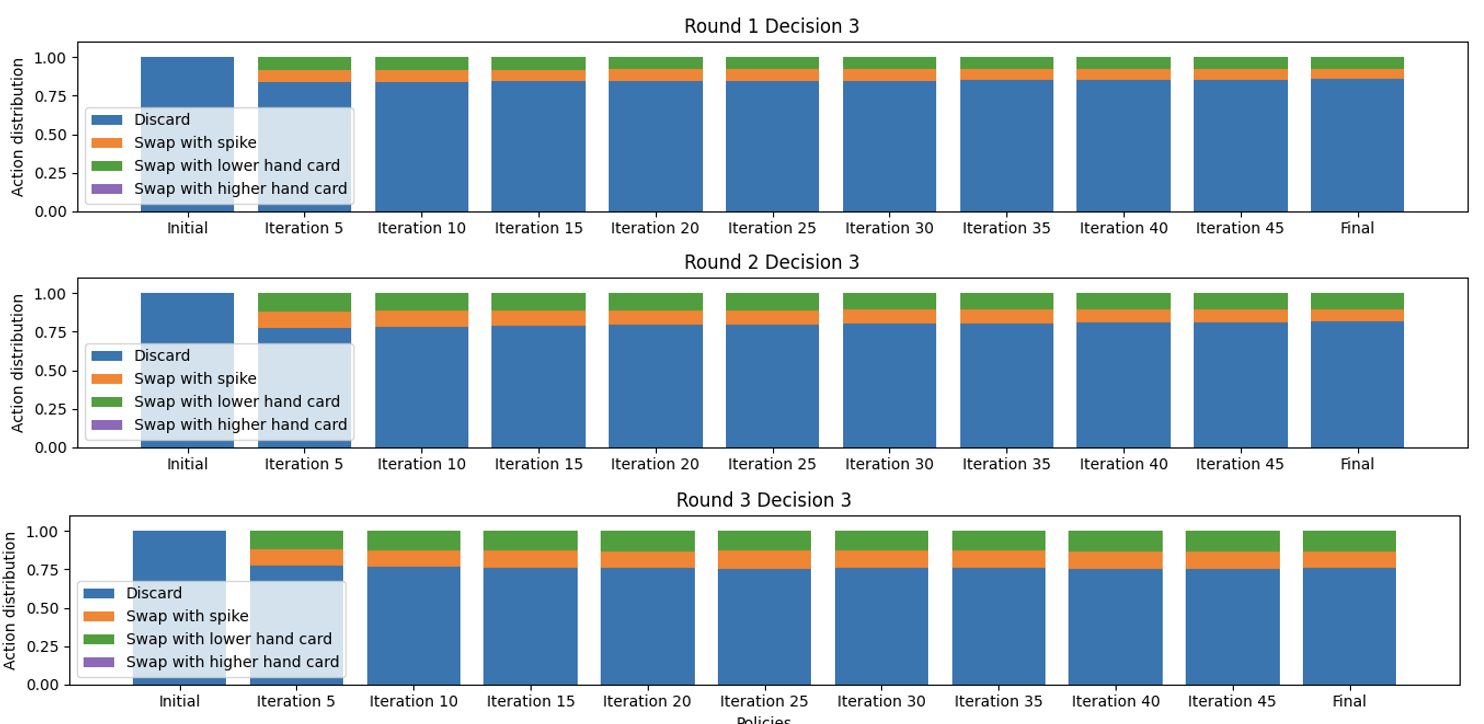
\includegraphics[width=\textwidth]{report/figures/weighted_r_d3.png}
        \caption{Action distribution for different policy iterations at Decision 3 with Weighted Reward Model and 2 players}
        \label{fig:weight_dec3_distribution}
    \end{figure}

\subsubsection*{Policy Distribution Plots Weighted Reward Model and Four Players}
    \begin{figure}[H]
    \centering
        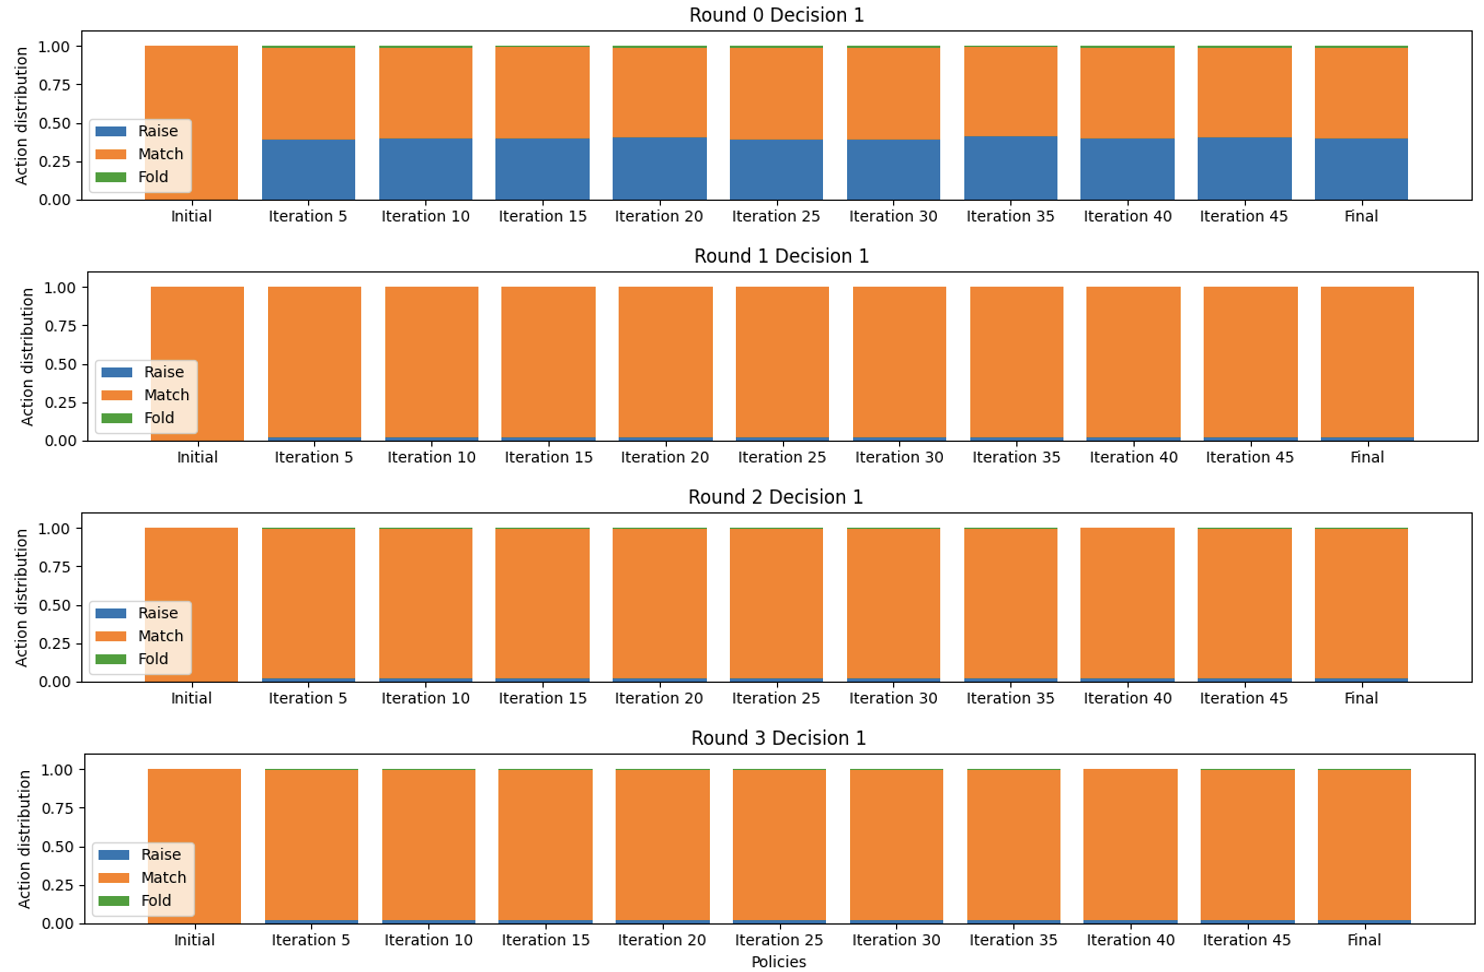
\includegraphics[width=\textwidth]{report/figures/4p_d1.png}
        \caption{Action distribution for different policy iterations at Decision 1 with Weighted Reward Model and 4 players}
        \label{fig:4p_dec1_distribution}
    \end{figure}
    
    \begin{figure}[H]
    \centering
        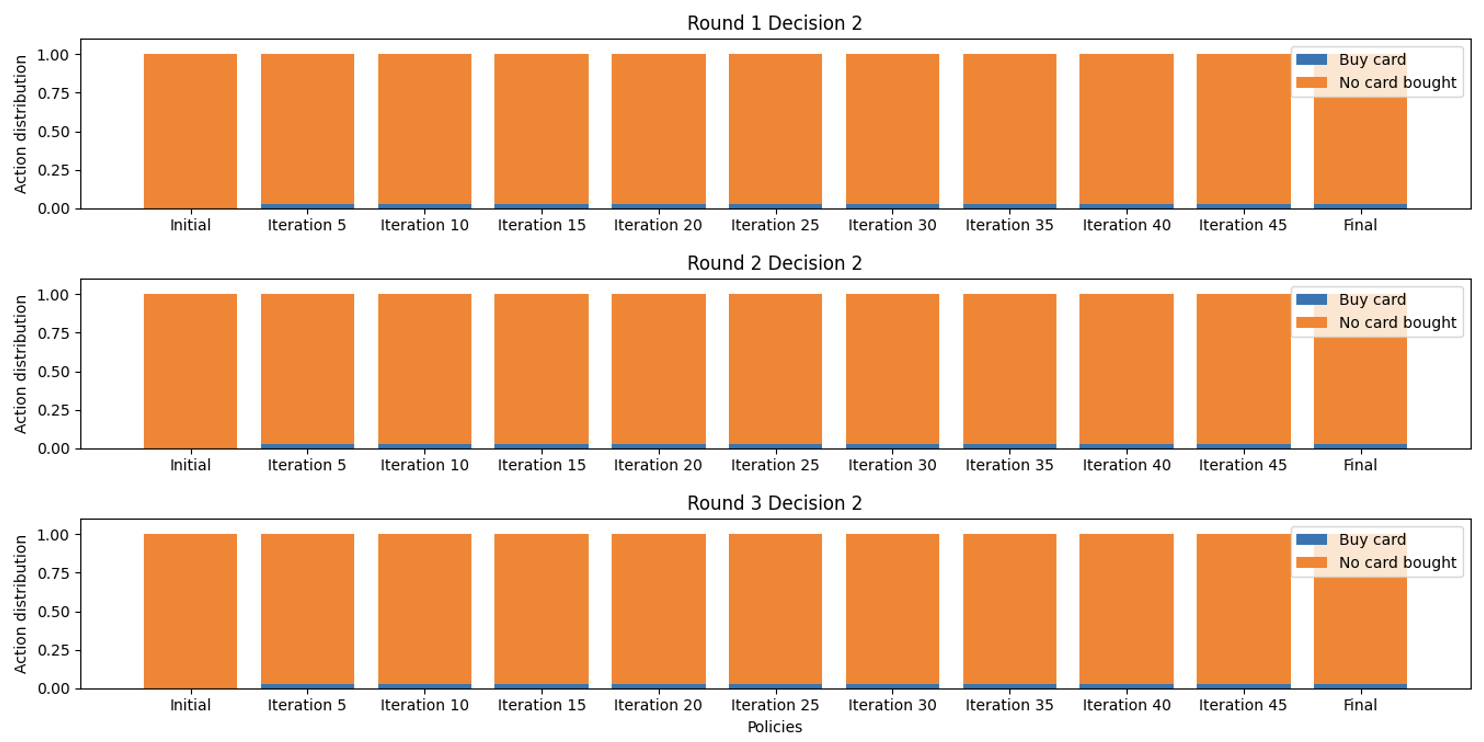
\includegraphics[width=\textwidth]{report/figures/4p_d2.png}
        \caption{Action distribution for different policy iterations at Decision 2 with Weighted Reward Model and 4 players}
        \label{fig:4p_dec2_distribution}
    \end{figure}
    
    \begin{figure}[H]
    \centering
        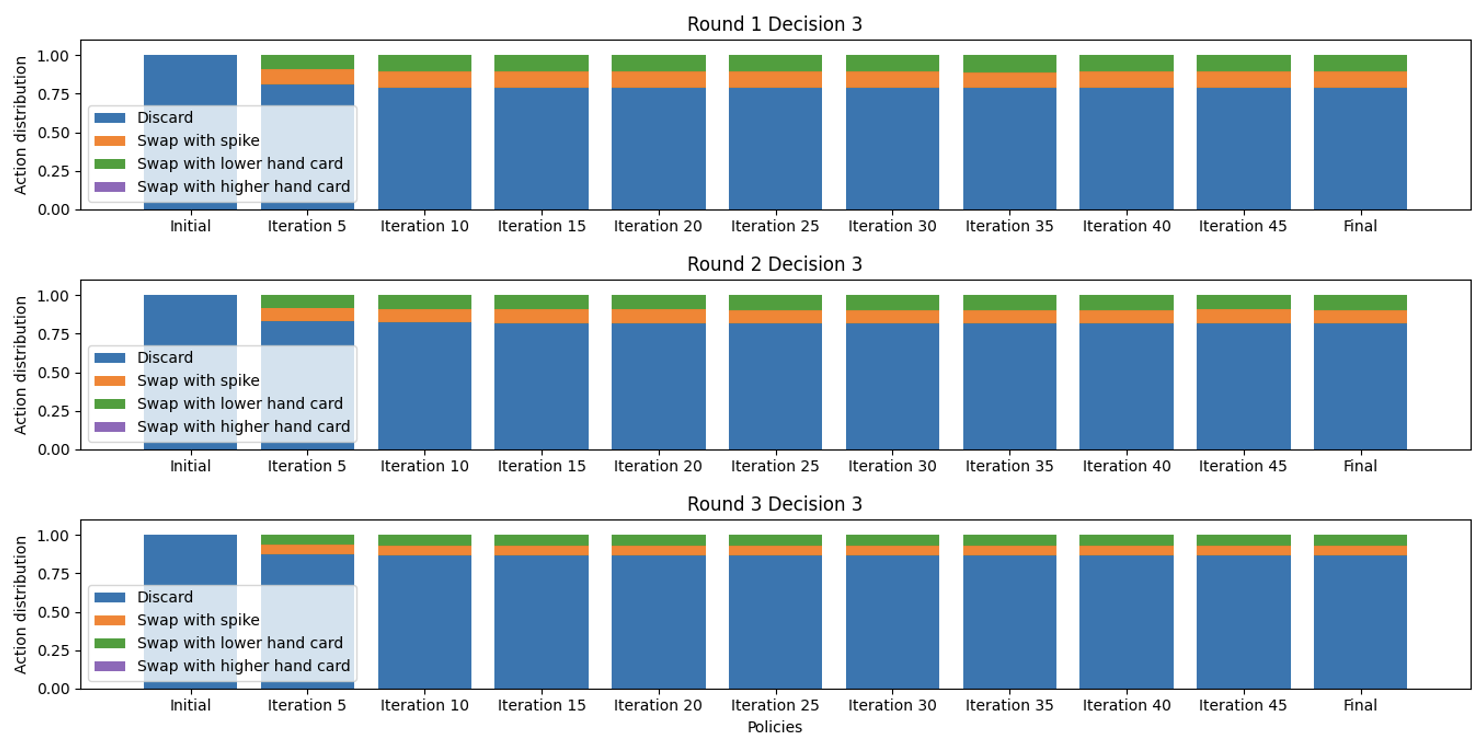
\includegraphics[width=\textwidth]{report/figures/4p_d3.png}
        \caption{Action distribution for different policy iterations at Decision 3 with Weighted Reward Model and 4 players}
        \label{fig:4p_dec3_distribution}
    \end{figure}
% Personal choice to do anything more


% \section{Headings: first level}
% \label{sec:headings}

% \lipsum[4] See Section \ref{sec:headings}.

% \subsection{Headings: second level}
% \lipsum[5]
% \begin{equation}
% 	\xi _{ij}(t)=P(x_{t}=i,x_{t+1}=j|y,v,w;\theta)= {\frac {\alpha _{i}(t)a^{w_t}_{ij}\beta _{j}(t+1)b^{v_{t+1}}_{j}(y_{t+1})}{\sum _{i=1}^{N} \sum _{j=1}^{N} \alpha _{i}(t)a^{w_t}_{ij}\beta _{j}(t+1)b^{v_{t+1}}_{j}(y_{t+1})}}
% \end{equation}

% \subsubsection{Headings: third level}
% \lipsum[6]

% \paragraph{Paragraph}
% \lipsum[7]



% \section{Examples of citations, figures, tables, references}
% \label{sec:others}

% \subsection{Citations}
% Citations use \verb+natbib+. The documentation may be found at
% \begin{center}
% 	\url{http://mirrors.ctan.org/macros/latex/contrib/natbib/natnotes.pdf}
% \end{center}

% Here is an example usage of the two main commands (\verb+citet+ and \verb+citep+): Some people thought a thing \citep{kour2014real, hadash2018estimate} but other people thought something else \citep{kour2014fast}. Many people have speculated that if we knew exactly why \citet{kour2014fast} thought this\dots

% \subsection{Figures}
% \lipsum[10]
% See Figure \ref{fig:fig1}. Here is how you add footnotes. \footnote{Sample of the first footnote.}
% \lipsum[11]

% \begin{figure}
% 	\centering
% 	\fbox{\rule[-.5cm]{4cm}{4cm} \rule[-.5cm]{4cm}{0cm}}
% 	\caption{Sample figure caption.}
% 	\label{fig:fig1}
% \end{figure}

% \subsection{Tables}
% See awesome Table~\ref{tab:table}.

% The documentation for \verb+booktabs+ (`Publication quality tables in LaTeX') is available from:
% \begin{center}
% 	\url{https://www.ctan.org/pkg/booktabs}
% \end{center}


% \begin{table}
% 	\caption{Sample table title}
% 	\centering
% 	\begin{tabular}{lll}
% 		\toprule
% 		\multicolumn{2}{c}{Part}                   \\
% 		\cmidrule(r){1-2}
% 		Name     & Description     & Size ($\mu$m) \\
% 		\midrule
% 		Dendrite & Input terminal  & $\sim$100     \\
% 		Axon     & Output terminal & $\sim$10      \\
% 		Soma     & Cell body       & up to $10^6$  \\
% 		\bottomrule
% 	\end{tabular}
% 	\label{tab:table}
% \end{table}

% \subsection{Lists}
% \begin{itemize}
% 	\item Lorem ipsum dolor sit amet
% 	\item consectetur adipiscing elit.
% 	\item Aliquam dignissim blandit est, in dictum tortor gravida eget. In ac rutrum magna.
% \end{itemize}


\bibliographystyle{unsrt}
\bibliography{references}  %%% Uncomment this line and comment out the ``thebibliography'' section below to use the external .bib file (using bibtex) .


%%% Uncomment this section and comment out the \bibliography{references} line above to use inline references.
% \begin{thebibliography}{1}

% 	\bibitem{kour2014real}
% 	George Kour and Raid Saabne.
% 	\newblock Real-time segmentation of on-line handwritten arabic script.
% 	\newblock In {\em Frontiers in Handwriting Recognition (ICFHR), 2014 14th
% 			International Conference on}, pages 417--422. IEEE, 2014.

% 	\bibitem{kour2014fast}
% 	George Kour and Raid Saabne.
% 	\newblock Fast classification of handwritten on-line arabic characters.
% 	\newblock In {\em Soft Computing and Pattern Recognition (SoCPaR), 2014 6th
% 			International Conference of}, pages 312--318. IEEE, 2014.

% 	\bibitem{hadash2018estimate}
% 	Guy Hadash, Einat Kermany, Boaz Carmeli, Ofer Lavi, George Kour, and Alon
% 	Jacovi.
% 	\newblock Estimate and replace: A novel approach to integrating deep neural
% 	networks with existing applications.
% 	\newblock {\em arXiv preprint arXiv:1804.09028}, 2018.

% \end{thebibliography}


\end{document}
